\documentclass[a4paper,12pt]{article}

\usepackage{amsmath,amssymb,multicol,tikz,enumitem}
\usepackage[margin=2cm]{geometry}
%\usetikzlibrary{calc}
\usepackage{amsmath}
\usepackage{amsthm}
\usepackage{thmtools}
\usepackage{hyperref}
\usepackage{enumerate}
\usepackage{xcolor}
\usepackage{fancyvrb}

\pagestyle{empty}

%\addtolength{\oddsidemargin}{1.125in}
%\addtolength{\evensidemargin}{1.125in}
%\addtolength{\textwidth}{-2.25in}

\newcommand\Q{\mathbf{Q}}
\newcommand\R{\mathbf{R}}
\newcommand\Z{\mathbf{Z}}

%\newcommand\answer[1]{}
%\newcommand\ans[1]{}
\newcommand\answer[1]{\\[5pt]{\color{blue}{#1}}\hfill{\color{blue}}\\[-5pt]}
\newcommand\ans[1]{{\color{blue}{#1}}}

\usepackage{array}
\newcolumntype{P}[1]{>{\centering\arraybackslash}p{#1}}

\newcommand\indd{${}$\hspace{20pt}}

\declaretheoremstyle[headfont=\normalfont\bfseries,notefont=\mdseries\bfseries,bodyfont = \normalfont,headpunct={:}]{normalhead}
%\declaretheorem[name={Uzdevums}, style=normalhead,numberwithin=section]{problem}
\declaretheorem[name={Uzdevums}, style=normalhead,numberwithin=section]{problem}

\setcounter{section}{1}

\setlength\parindent{0pt}

\renewcommand{\figurename}{Attēls}

\begin{document}

\begin{center}
\parbox{3.5cm}{\flushleft\bf Dažāda skaitļu teorija} \hfill {\bf\LARGE Sacensības 2021/2022 \#01} \hfill \parbox{3.5cm}{\flushright\bf 2021-09-20} \\[2pt]
{\rm\footnotesize Par šo LU NMS atbalstīto pasākumu\\ atbild {\tt kalvis.apsitis@gmail.com}.}
\end{center}

%Atbildes uz šī testa uzdevumiem ir nelieli veseli skaitļi. Lai gan dažos gadījumos aprēķini uz datora
%var noderēt, tomēr visi uzdevumi ir atrisināmi saprātīgā laikā uz papīra līdzīgi kā olimpiādēs.

%\hrule\vspace{2pt}\hrule
\hrule

%%%%%%%%%%%%%%%
%%% 01 %%%%%%%%
%%%%%%%%%%%%%%%
\vspace{10pt}
\begin{problem}
%2022.1.1
\mbox{}\\
Dots taisnstūra paralēlskaldnis $ABCDA_1B_1C_1D_1$ ar izmēriem $30 \times 72 \times 100$, tas salikts no vienības kubiņiem
ar izmēriem $1 \times 1 \times 1$.
Cik daudzus no šiem kubiņiem šķērso dia\-go\-nā\-le $AC_1$?
(Ja diagonāle tikai pieskaras vienības kubiņa virsotnei vai šķautnei, to neuzskata par šķērsošanu.)
\answer{

{\bf Atbilde.} $\mathtt{186}$

LKD(30,72,100) = 2, tāpēc lielā paralēlskaldņa vietā var aplūkot divus divreiz mazākus ar izmēriem
$15 \times 36 \times 50$.
Ja visi skaitļi (15, 36, 50) būtu savstarpēji pirmskaitļi, tad diagonālei vajadzētu
šķērsot $(15 + 36 + 50) - 2 = 99$ kubiņus, lai no kreisā, apakšējā, priekšējā kubiņa
tiktu līdz labajam, augšējam, aizmugurējam kubiņam (var saskaitīt, cik reizes jāpalielina
kāda no koordinātēm $x$, $y$, vai $z$, lai to izdarītu).

Tomēr ir lielākie kopīgie dalītāji: $\mbox{LKD}(15,36) = 3$,
$\mbox{LKD}(15,50) = 5$, $\mbox{LKD}(36,50) = 2$ (toties $\mbox{LKD}(15,36,50) = 1$).


}
\end{problem}


%%%%%%%%%%%%%%%
%%% 02 %%%%%%%%
%%%%%%%%%%%%%%%
\vspace{10pt}
\begin{problem}
%2022.1.2
\mbox{}\\



Aplūkosim $700$ skaitļu reizinājumu $(2-1)(4-1)\ldots{}(2^{700} - 1)$:
\[ N = \prod\limits_{k=1}^{700} \left( 2^k - 1 \right). \]
Apzīmēsim ar $\nu_5(N) = a$ lielāko skaitļa $5$ pakāpi, ar ko dalās $N$
(t.i. $N$ dalās ar $5^{a}$, bet vairs nedalās ar $5^{a+1}$).
Līdzīgi apzīmējam ar $\nu_7(N)$ lielāko skaitļa $7$ pakāpi, ar ko dalās $N$
(to sauc par skaitļa $N$ $7$-valuāciju).

Atrast starpību:
\[ \Delta = \nu_5(N) - \nu_7(N). \]

%Ierakstīt atbildē veselu skaitli $\Delta$: abu valuāciju starpību.

\vspace{20pt}
{\bf Atbilde.} $\mathtt{-52}$

Pamatosim, ka $\Delta = \nu_5(N) - \nu_7(N) = 218 - 270 = -52$.

Rakstām kāpinātāja pacelšanas lemmu:

{\bf Lemma.}


Šis testa jautājums ir atsauce uz 2019.g.\ Starpautiskās olimpiādes uzdevumu:

{\bf IMO2019.P4.} Atrast visus naturālo skaitļu $(k,n)$ pārus, kuriem izpildās
\begin{equation}
\label{eq:imo2019p4}
k! = (2^n - 1)(2^n - 2)(2^n - 4) \cdots (2^n - 2^{n-1}).
\end{equation}

Zinot kāpinātāja pacelšanas lemmu, var pamanīt, ka vienādības (\ref{eq:imo2019p4}) labajā
pusē ir izteiksme, kas (pietiekami lieliem $n$) dalās ar augstāku skaitļa $7$ pakāpi
nekā skaitļa $5$ pakāpi. Tāpēc šīs izteiksmes vērtība nevar būt $k!$ nevienam
pietiekami lielam $k$, jo faktoriālam $\nu_5(n) \geq \nu_7(n)$ katram $n$.
Pateicoties Ležandra formulai - \url{https://bit.ly/30N0EtL}.

\end{problem}



%%%%%%%%%%%%%%%
%%% 03 %%%%%%%%
%%%%%%%%%%%%%%%
%\vspace{10pt}
\clearpage
\begin{problem}
%2022.1.3
\mbox{}\\

Attēlā dots "Kantora kvadrants", kas režģa punktus $(0,0)$, $(1,0)$ $(0,1)$, $\ldots$ pēc kārtas aizpilda ar
skaitļiem  $0,1,2,\ldots$.
Šajā kvadrantā katram veselam nenegatīvam skaitlim ir divas "Dekarta koordinātes" (kas arī ir veselas nenegatīvas).
Piemēram, skaitļa $17$ koordinātes ir $(x,y) = (3,2)$.

\begin{figure}[!htb]
\center{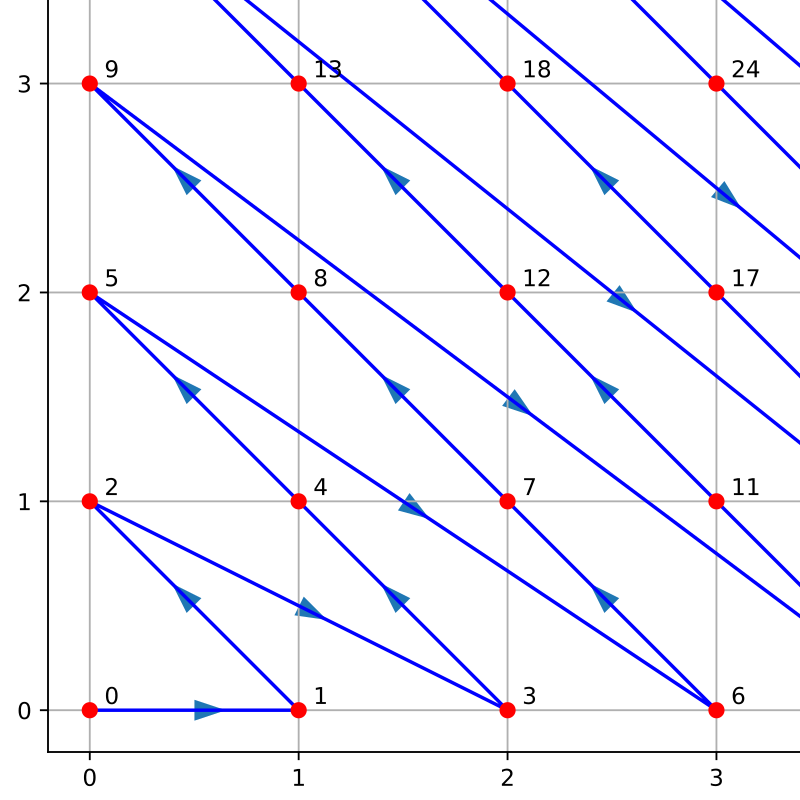
\includegraphics[width=2.7in]{online-competition-2021-09-20/pairing_function.png}}
\caption{\label{fig:pairing_function} Kantora kvadrants.}
\end{figure}

Atzīmēsim šajā kvadrantā kvadrāttrinoma  ${\displaystyle f(z) = \frac{z^2 + z + 356}{2}}$ vērtības
veseliem argumentiem $z$. Zināms, ka visas (izņemot galīgu skaitu) no šīm vērtībām
atrodas uz horizontālas taisnes: tām $y$ koordināte ir viena un tā pati.
Atrast šo $y$ koordināti.

\answer{

{\bf Atbilde.} $\mathtt{178}$.

TBD
}
\end{problem}




%%%%%%%%%%%%%%%
%%% 04 %%%%%%%%
%%%%%%%%%%%%%%%
\vspace{10pt}
\begin{problem}
%2022.1.4
\mbox{}\\

$F_n$ apzīmē Fermā skaitli: ${\displaystyle F_n = 2^{2^n} + 1}$, kur $n = 0,1,2,\ldots$.

Zināms, ka pirmskaitlis $p$ ir ar sekojošu īpašību:
$F_{n+3} - F_{n}$ dalās ar $p$ visiem naturāliem $n$ (iespējams, izņemot galīgu skaitu
$n$ vērtību).

Atrast kādu šāda pirmskaitļa $p$ piemēru.

\answer{

{\bf Atbilde.} $\mathtt{2}$ (un arī $\mathtt{29}$, $\math{43}$).


Ir viena triviāla atbilde $p = 2$ (jo visas Fermā skaitļu starpības dalās ar $n$).
Ir arī $\mathtt{29}$ (arī $43$ un daži citi piemēri).




%Loop detected (p,i)=(29,3)
%Loop detected (p,i)=(43,3)
%Loop detected (p,i)=(113,3)
%Loop detected (p,i)=(449,3)

}
\end{problem}




%%%%%%%%%%%%%%%
%%% 05 %%%%%%%%
%%%%%%%%%%%%%%%
\vspace{10pt}
\begin{problem}
%2022.1.5
\mbox{}\\

% https://handwiki.org/wiki/Prime_omega_function

Naturālam skaitlim ar sadalījumu pirmreizinātājos
$n = p_1^{a_1}p_2^{a_2}\ldots{}p_k^{a_k}$ definējam $\omega(n) = k$:
tas ir visu skaitļa $n$ dažādo pirmreizinātāju skaits.
(Piemēram, $\omega(1) = 0$, $\omega(2) = \omega(3) = \omega(5) = \ldots = 1$,
$\omega(4) = \omega(8) = 1$, $\omega(6) = \omega(12) = 2$, $\omega(210) =4$, utml.)

Atrast sekojošas summas vērtību:

\[ 2^{\omega(d_1)} + 2^{\omega(d_2)} + 2^{\omega(d_3)} + \ldots + 2^{\omega(d_k)}, \]
kur $d_1,\ldots, d_k$ ir visi skaitļa $2016$ pozitīvie dalītāji.

\answer{

{\bf Atbilde.} $\mathtt{165}$

Since $2016^2 = (2^5 \cdot 7 \cdot 3^2)^2 = 2^{10} 3^4 7^2$,
it has $11 \cdot 3 \cdot 3 = 165$ positive divisors.


}
\end{problem}




%%%%%%%%%%%%%%%
%%% 06 %%%%%%%%
%%%%%%%%%%%%%%%
\clearpage
%\vspace{10pt}
\begin{problem}
%2022.1.6
\mbox{}\\

Atvērtas iekavas izteiksmē $(x + y)^{2020}$ un polinomā sagrupēti līdzīgie locekļi:

\[ (x + y)^{2020} = x^{2020} + 2020 x^{2019}y + \ldots  + 2020 x y^{2019} + y^{2020}. \]

Atrast, cik daudzi no šī polinoma koeficientiem dalās ar $2020$.

\answer{


{\bf Atbilde.} $\mathtt{1718}$.

TBD

}
\end{problem}



%%%%%%%%%%%%%%%
%%% 07 %%%%%%%%
%%%%%%%%%%%%%%%
\vspace{10pt}
\begin{problem}
%2022.1.7
\mbox{}\\

% https://artofproblemsolving.com/community/c6h2342235p18895780

Cik ir pirmskaitļu $p < 100$ ar sekojošu īpašību:
Jebkuriem veseliem $x,y$
no dalāmības $p \mid x^2 + y^2$ izriet $p \mid xy$?
(T.i. $x^2 + y^2$ var dalīties ar $p$ vienīgi tad, ja $xy$ dalās ar $p$.)

\answer{

{\bf Atbilde.} $\mathtt{13}$.

Tie ir visi pirmskaitļi formā $4n +3$:

\[ 3, 7, 11, 19, 23, 31, 43, 47, 59, 67, 71, 79, 83. \]

Šādiem pirmskaitļiem $p$, ja vienādojumu $x^2 \equiv a \pmod{p}$ var
atrisināt, tad vienādojumu $x^2 \equiv -a \pmod{p}$ nevar atrisināt
(vienīgais izņēmums ir tad, ja $a = 0$).

}
\end{problem}



%%%%%%%%%%%%%%%
%%% 08 %%%%%%%%
%%%%%%%%%%%%%%%
\vspace{10pt}
\begin{problem}
%2022.1.8
\mbox{}\\

Dots naturāls skaitlis $n$. Apzīmēsim ar $\nu_2(n)$ lielāko divnieka pakāpi, ar kuru tas dalās.
(Piemēram, $\nu_2(1) = \nu_2(3) = \nu_2(5) = \ldots = 0$, $\nu_2(2) = \nu_2(6) = \nu_2(10) = \ldots = 1$,
$\nu_2(4) = \nu_2(12) = \ldots = 2$.)

Atrast mazāko skaitli $n$, kuram $n - \nu_2(n!)$ un $(n+1) - \nu_2((n+1)!)$ ir divi dažādi veseli
skaitļi, kas abi dalās ar $3$.

\answer{

{\bf Atbilde.} $\mathtt{111}$.

Skaitļa $111$ binārais pieraksts ir $\mathtt{1101111}_2$, bet
skaitļa $112$ binārais ieraksts ir $\mathtt{1110000}_2$.

}
\end{problem}


%%%%%%%%%%%%%%%
%%% 09 %%%%%%%%
%%%%%%%%%%%%%%%
\vspace{10pt}
%\clearpage
\begin{problem}
%2022.1.9
\mbox{}\\

% Bērziņa grāmata 4.1.5

Dots vienādojums veselos skaitļos:

\[ x^4 - 12 y^4 = 24. \]

Atrast naturālu skaitli $m$, kas ir {\em pretrunas modulis}
šim vienādojumam: Jebkuram veselu skaitļu pārim $(x,y)$
izteiksmes $x^4 - 12 y^4$ un $24$ dod atšķirīgus atlikumus, dalot ar $m$
(tātad tās nevar būt vienādas).
Ja tādi $m$ ir vairāki, centieties atrast mazāko iespējamo.

\answer{

{\bf Atbilde.} $\mathtt{13}$.


TBD

}
\end{problem}



%%%%%%%%%%%%%%%
%%% 10 %%%%%%%%
%%%%%%%%%%%%%%%
\vspace{10pt}
\begin{problem}
%2022.1.10
\mbox{}\\

Ciparu virkni $D = d_{n-1}d_{n-2}\ldots{}d_0$ sauksim par {\em stabilu skaitļa
nobeigumu}, ja jebkuram naturālam skaitlim $m$, kas beidzas ar virkni $D$,
arī jebkura tā pakāpe $m^k$ beidzas ar šo pašu virkni $D$.
Atrast to stabilo skaitļa nobeigumu $D$, kas sastāv no astoņiem cipariem
un ir lielākais iespējamais (kā astoņciparu skaitlis).

\answer{

{\bf Atbilde.} $\mathtt{87109376}$.

Ir arī trīs citas atbildes: $\math{00000000}$, $\math{00000001}$ un
$\math{12890625}$, bet tie ir mazāki skaitļi.

Stabilas ciparu virknes var konstruēt ar indukciju - sākot ar skaitļa beigām. 
Ir, teiksim, četras stabilas virknes 1 cipara garumā: {\tt 0,1,5,6} --
kāpinot kvadrātā skaitli, kas beidzas ar kādu no šiem cipariem, arī rezultāts beigsies ar to pašu. 

No diviem cipariem tieši tāpat var izveidot četras stabilas virknes: {\tt 00, 01, 25, 76}.
No trim cipariem attiecīgi virknes {\tt 000, 001, 376, 625}. 

{\bf Kāpēc virkņu dotajā garumā nevar būt vairāk kā četras?}

Pamatosim šo ar indukciju. Pieņemsim, ka $n$ ir lielākais naturālais skaitlis, 
kuram stabilo virkņu garumā $n$ ir tieši četras. 
Jebkura stabila virkne garumā $n+1$ būs tāda, ka tās pēdējie $n$ cipari arī veido 
stabilu virkni. Pamatosim, ka $n$-ciparu virknes (ko apzīmēsim ar skaitli $x$) 
kreisajā pusē jaunu ciparu var "pieaudzēt"
ne vairāk kā vienā veidā tā, lai virkne joprojām būtu stabila. 

No pretējā -- pierakstām skaitlim $x$ priekšā divus dažādus ciparus: $d_a$ un $d_b$ 
un pieņemam, ka jaunās virknes joprojām ir stabilas.

\[ \left\{ \begin{array} 
(10^n d_a + x)^2 \equiv 10^n d_a + x \pmod 10^{n+1}\\
(10^n d_b + x)^2 \equiv 10^n d_b + x \pmod 10^{n+1}\\
\end{array} \right.
\]


}
\end{problem}


%%%%%%%%%%%%%%%
%%% 11 %%%%%%%%
%%%%%%%%%%%%%%%
\vspace{10pt}
\begin{problem}
%2022.1.11
\mbox{}\\

% BW.TST.2015.14

Ar $S(a)$ apzīmēsim skaitļa $a$ ciparu summu.
Atrast iespējami mazu naturālu $n$, kuram
\[ \frac{S(n^2)}{S(n)} = 10. \]

\answer{

{\bf Atbilde.} $\mathtt{10111111111}$.

{\bf Skaitļa atrašana.}
Skaitli var kāpināt kvadrātā, izmantojot skolas algoritmu (reizināšanu stabiņā).
Ja vajag iegūt attiecības $\frac{S(n^2)}{S(n)} = d$ (kur $d = 1,\ldots,9$),
var izvēlēties $n=1$, $n=11$, $n=111$, utt. līdz pat $n=111\,111\,111$.

Savukārt, ja $\frac{S(n^2)}{S(n)} = 10$, tad
skaitlis $n = 1111111111$ vairs neapmierina nosacījumu: to kāpinot kvadrātā rodas
divi pārnesumi (katrā no pārnesumiem ciparu summa vienā skaitļu šķirā samazinās par $10$, lai
nākamajā skaitļu šķirā palielinātos par $1$ -- t.i. kopīgā ciparu summa samazinās par $9$).

\begin{verbatim}
          1111111111
        * 1111111111
		------------
          1111111111
         1111111111
        1111111111
       1111111111
      1111111111
     1111111111
    1111111111
   1111111111
  1111111111
 1111111111
---------------------
 1234567900987654321
\end{verbatim}

Tā kā notiek divi pārnesumi, iegūtā skaitļa ciparu summa ir $S(n^2) = 100 - 2 \cdot 9 = 82$,
kas ir mazāk nekā $10\cdot S(n) = 100$.

Aplūkojam mazāko $11$-ciparu skaitli, kuram ir $10$ nenulles cipari: $n = 10111111111$.
Kāpinot to kvadrātā, izrādās, ka pārnesumu nav vispār:
$n^2 = 102234567898987654321$. Ciparu summa $S(n^2) = 100$, kas tiešām ir desmit reizes lielāka par $S(n)$.

{\bf Optimalitātes pamatojums.}



}
\end{problem}



%%%%%%%%%%%%%%%
%%% 12 %%%%%%%%
%%%%%%%%%%%%%%%
\vspace{10pt}
\begin{problem}
%2022.1.12
\mbox{}\\

Matemātiķis $A$ iečukstēja ausī matemātiķiem $B,C,D$ un $E$ četrus pēc kārtas sekojošus divciparu skaitļus $n,n+1,n+2,n+3$.
(Pašiem $B,C,D,E$ nav zināms, kuram iečukstēts lielākais, mazākais utml.)
Matemātiķis turklāt pateica viņiem visiem, ka visi skaitļi ir pēc kārtas sekojoši, ka
viens no kopas $S = \{ n,n+1,n+2,n+3 \}$
skaitļiem dalās ar $6$, bet kāds cits skaitlis dalās ar $7$.
Matemātiķis $A$ tad jautāja četriem pārējiem, vai iespējams izsecināt $n$ vērtību, visi reizē atbildēja "Nē".
Bet tūlīt pēc tam katrs no viņiem jau zināja $n$ vērtību.

Atrast lielāko iespējamo divciparu skaitli $n$, kuram izpildās aprakstītā īpašība.
\answer{

{\bf Atbilde.} $\mathtt{89}$.

Pamatosim, ka šie divciparu skaitļi ir $\{ 89,90,91,92 \}$ (tātad mazākais no viņiem ir $n=89$).

Ir nepieciešams, lai
abi vidējie skaitļi būtu tādi, ka viens no tiem dalās ar $6$, bet otrs ar $7$
(nav svarīgi, kurā secībā). Ja ar $6$ vai ar $7$ dalās kāds no malējiem skaitļiem (piemēram, $n$
vai $n+3$), tad tas matemātiķis, kuram iečukstēja skaitli intervāla otrajā galā (attiecīgi $n+3$ vai $n$),
pārbaudot dalāmību ar $6$ un ar $7$ varēs viennozīmīgi atjaunot visu intervālu
$S = \{ n,n+1,n+2,n+3 \}$.

Izrakstām visus tos blakusesošos pārus $(n+1,n+2)$, kur viens no skaitļiem dalās ar $6$, bet otrs ar $7$:

\begin{verbatim}
35,36
48,49
77,78
90,91
\end{verbatim}

Lielākais no šiem pāriem ir $(n+1,n+2) = (90,91)$. Tātad lielākais iespējamais
$n$ ir $n=89$ un četri iečukstētie skaitļi ir $\{ 89,90,91,92 \}$.


{\small
Sk. arī {https://bit.ly/3jqQRjq} -- AIME2021_2P11; cits šī uzdevuma variants.
}
}
\end{problem}






\end{document}









